\chapter{Pre and post processing work preparation}
\label{Chapter2}

\section{Introduction}

This chapter focuses on the preparation of the tests and the tools used to obtain results. It explains in detail the equipment used to carry out the tests and the preparation made for them. A section is devoted to the application of the DIC method and the proper use of MatchID. It explains some important parameters such as subset size, step size in order to make the DIC analysis as accurate as possible.
Finally, two fracture analysis methods are presented. A Python code was developed for both methods, and this section also allows a comparison of these two methods and a judgment on which is the most effective.

\section{Tools used during the test}

\subsection{MMCG test piece}

The MMCG test piece was developed by \cite{MoutouPitti2008}. However, the specimens tested at the University of Lisbon are not of the same dimensions. After carefully measuring the specimens, it turns out that they have the same dimensions as the specimens studied by \cite{Odounga2018phd}. Below are the dimensions of the specimens that will be tested figure \ref{fig:fig23}:


\begin{figure}[htp]
	\centering
	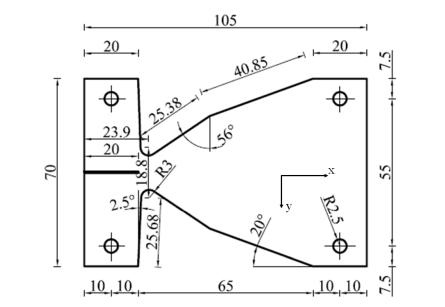
\includegraphics[width=8cm]{fig23}
	\caption{Dimensions of the tested MMCG specimen}
	\label{fig:fig23}
\end{figure}

\subsection{Characteristic of the Wood used}

For the tests conducted in this thesis, the European species chosen is the silver fir. This coniferous tree is a derivative of needle trees.  Present on north hemisphere, it is a softwood as Pines or others old trees. Its name originates from its white color and its circumference ranges from 50 to 80 cm. CIRAD data shows a density of 0.45 to 0.60, a SFP of about 30$\%$, and a compressive strength of 41MPa. The tangential shrinkage is significant at 8.7$\%$, whereas the radial shrinkage is at 4$\%$. The wood of the Silver Fir is commonly used for framing, columns, and light framing due to its strength, although it must be treated to prevent fungal and insect attacks. The main concern with this wood is the presence of a water pocket in the tree, as well as its tendency to split, which may limit the use of certain connectors in construction.

In order to compare the future results of tensile tests with the literature review, we need to know some characteristics of our sample.
We therefore decided to measure its weight, density, and moisture content.
The samples were first weighed just before the test. This measurement is called $M_H$. 
This allows us to know the mass of the wood samples during the test.
The density of the wood can also be deduced from the volume of the sample and its mass.
The sample was previously drawn in AutoCAD. The theoretical surface of the sample can therefore be known directly and multiplied by the thickness.
We can therefore deduce the density of each sample by applying the formula $\rho=M/V$.
After testing, the specimens are placed in an oven at 100 degrees until the $M_C$ mass is stabilised. Two specimens were placed in an oven during 73 hours. Different measurements were taken until a constant mass of the specimen was obtained.
The moisture content can then be determined by applying the equation \ref{eq:HI}.
Finally, we have the mass, the density and the moisture content to compare our results with the literature review in table \ref{tab:Tabmean}.

\begin{table}[h]
	\centering
	\begin{tabular}{c c }
		\multicolumn{1}{l}{} & \multicolumn{1}{l}{Average value} \\
		\multicolumn{1}{c}{\cellcolor[HTML]{F8CBAD}MH} & 29.83   g \\
		\multicolumn{1}{c}{\cellcolor[HTML]{F8CBAD}V} & 6916 cm3 \\
		\multicolumn{1}{c}{\cellcolor[HTML]{F8CBAD}$\rho$} & 431.3 kg/m3 \\
		\multicolumn{1}{c}{\cellcolor[HTML]{F8CBAD}HI} & 10.3 \% \\
	\end{tabular}
	\caption{Characteristics of MMCG Silver Fir}
	\label{tab:Tabmean}
\end{table}

\subsection{Arcan model and final grips}

To perform the tests, a steel Arcan system must be designed. Indeed, this part allows to connect the 2MCG wood specimen to the press. In order to create this grip we must first take into account the dimensions of the 2MCG specimen available at Nova School described in figure \ref{fig:fig23}. The shape of the Arcan system must also allow good visibility for the propagation of the crack. Figure \ref{fig:fig24} shows the Arcan device that we will use, which was inspired from the thesis of \cite{Odounga2018phd}.


\begin{figure}[htp]
	\centering
	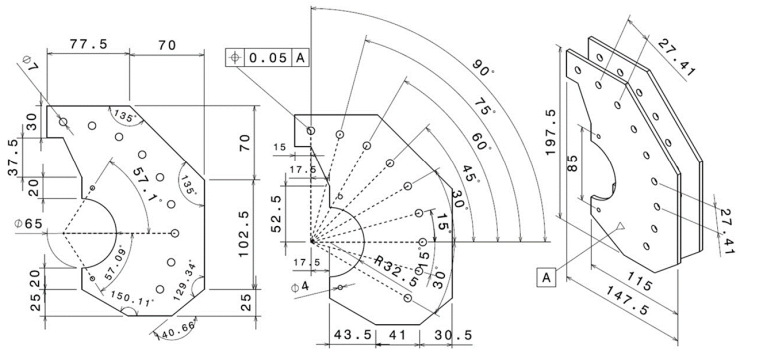
\includegraphics[width=15cm]{fig24}
	\caption{Size of the Arcan fastening system, \cite{Odounga2018phd}}
	\label{fig:fig24}
\end{figure}

The fixing holes for the wooden specimens have a diameter $\Phi= 4 mm$, and the loading holes have a diameter $\Phi = 7 mm$. These fixing holes were drilled in order to be able to load the specimen with different angular values of the angle in relation to the vertical direction in order to activate different failure modes depending on the load angle. To connect the Arcan system to the press, a piece had to be created, as shown in figure \ref{fig:fig25}.


\begin{figure}[htp]
	\centering
	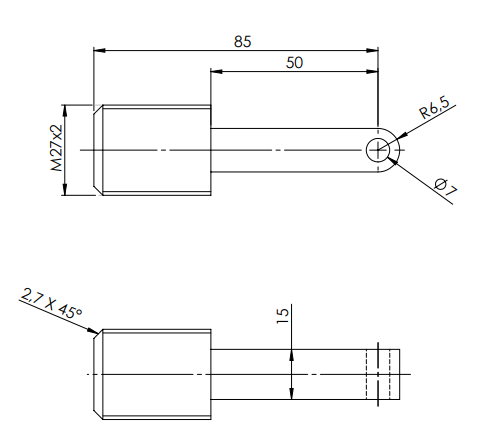
\includegraphics[width=6cm]{fig25}
	\caption{Bolt for connecting the press and the Arcan System}
	\label{fig:fig25}
\end{figure}

This part has a hole of the same size as the holes of the Arcan system in order to connect them. Moreover the head of the connector is 27mm in diameter, and the thread has a 2mm pitch to connect to the press. Before sending the technical drawings to a company, a 3D printer was used to verify that the system worked properly. It was then necessary to draw the assembly on Solidworks in order to print the assembly and send the technical drawings. Figure \ref{fig:fig26} shows the assembled device in Solidworks. Solidworks is a 3D modeler owned by Dassault using parametric design, which generates 3 types of files related to three basic concepts: the part, the assembly, and the drawing.


\begin{figure}[htp]
	\centering
	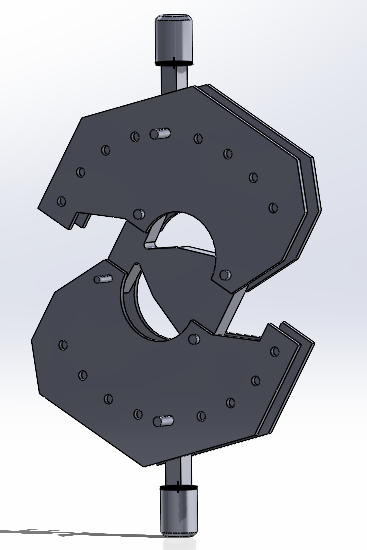
\includegraphics[width=7cm]{fig26}
	\caption{Assembled device in Solidworks}
	\label{fig:fig26}
\end{figure}

It has been shown in previous work such as \cite{Odounga2018phd} that one of the main problems with the MMCG specimen is the small distance between the holes and specimen extremities. This implies several cracks in the heel between the hole and the extremity of the sample which prevent observation and analysis of the fracture. One solution proposed is the use of washers which could be glued or to strength screw the nut. Indeed, by applying compressive stress on each side of the sample, it reduces the stress applied to the holes and distributes the load over a wider area.

\subsection{Hydraulic press used}

To determine experimental parameters like the load speed or the frequency of the camera recording, it was important to read previous works on the subject and determine which engines will be used to proceed the experiments. The press used for the tests is a Landmark Servohydraulic Test Systems model 661.21B-03  from MTS. It is capable of exerting a maximal applied load of 100 kN (figure \ref{fig:fig27}).
In the work of \cite{Ostapska2021} the load speed recommended was about $0.1\ mm\ {min}^{-1}$ and the record was made at a frequency of 5 Hz, so 5 images per seconds. In the work of \cite{Mambili2018} the record was made at a frequency of 10 Hz and the load speed was about 0.3 mm/min with a pre-load of 100N. It should be remembered that this press is also chosen because of its ability to load the specimens with a constant time displacement. Indeed, it was explained that this work will use the complacency method to compare the results.

This MTS Hydraulic Press works with a cooler fluid. Indeed, a tank full of fluid mixed to water and a cooler system send this fluid mix to the press as visible on \ref{fig:fig27}. Then, a hydraulic supply from MTS sends this liquid to the press itself. It is the model 506.02 serie 22 coupled with the Vickers DG4V-3-2A. Then the pressure is created thanks to the Hydraulic Service Manifold part from MTS company, model 234.11. Finally, a servo valve MOOG A076-263c increase the pressure to allow the hydraulic press operation. It is a high performance valve that drives a dry torque motor. Then a MTS load cell (661-21B-03) allows to follow the displacement of the hydraulic press.


\begin{figure}[htp]
	\centering
	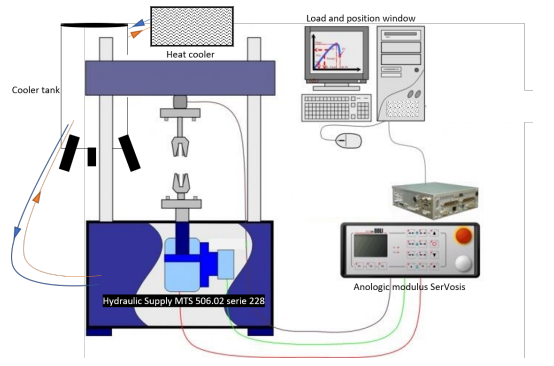
\includegraphics[width=10cm]{fig27}
	\caption{Hydraulic Press components allowing it use, \cite{MALFAIT2021}}
	\label{fig:fig27}
\end{figure}

To avoid displacement of the specimens, a preload is applied to the wood specimen. In the tests performed by \cite{MALFAIT2021} this preload was ignored to avoid negative loading values. An offset was applied to the P-$\delta$ to avoid these negative values which do not make sense. By ignoring this first loading, all results are truncated and the impacts on other parameters such as the energy release rate is disastrous. 
To remedy this problem, it is necessary to examine the load of the hydraulic press before it is used. This value, even if it is negative, will be subtracted from all the others, which will give the preload. Another solution is to continue testing, even after the propagation in the ZOI has ended. Indeed, the value of the load at the end of the test, on a collapsed specimen, will be equal to zero, even if the zero value is negative.

\section{Research and understanding of the parameters of the DIC method}

\subsection{Preparation of the DIC method}

It is possible to process the images with different software. This image processing will allow to obtain maps of deformations and displacements. For this work will be used MatchID a correlation image software and Python.
In our case, the quantity of interest is the crack length a as a function of the applied force F. The field of view ( FOV), the position envelope for hardware and if the test is a 2D-DIC or a stereo DIC are parameters to take into account. In our case, a 2D-DIC is suitable because the test piece is assumed to be planar and perpendicular to the camera optical axis. The DIC pattern is one important parameter. All the specimens are painted to obtain a speckle pattern suitable for image correlation. A thin layer of white paint is first added using a mate spray, followed by a diffuse distribution of black paint to create a unique local pattern across the ZOI at the crack tip. Before starting the test, some parameters must be set on MatchID.grab or other software if the camera is not registered in MatchID. It is possible to vary parameters such as the exposure time. The speckle pattern is an image composed of black and white dots. By varying the exposure time, the speckle pattern will have a greater or lesser range of gray (from 0 to 255). On the other hand, a longer exposure time will result in color saturation. Then, it is important to adjust the quality of the speckle using two parameters, the focus and the aperture. With some cameras, it is sometimes impossible to adjust the focus. It is therefore necessary to play with the distance camera-specimen.

\subsection{MatchID}

After calibration and recording of the tests, the datas must be processed. Several steps are necessary:

\begin{itemize}
	\item Choose a reference image that corresponds to the first image of the test 
	\item Select multiple deformed images
	\item Define the zone of interest (ZOI) in which the crack propagates
	\item Define the analysis parameters of the ZOI
	\item Start the DIC analysis
	\item Exploit the results
\end{itemize}

Despite the progress and increasing use of DIC, the technique is still not standardized. It is emphasized that extrinsic and intrinsic DIC setup parameters, such as subset size, subset step, strain gauge window, shape functions, or correlation criterion, can have a considerable influence on the calculated strain fields, producing spatial resolution and resolution values that can differ by at least an order of magnitude \cite{DICguide2018}. The next paragraph will try to explain some of them. 

\begin{itemize}
	\item The \textbf{correlation criterion} defines the matching criterion that will be adopted in order to determine the optimum corresponding point. \cite{MALFAIT2021}  used the criterion ZNSSD. It is a least-square-based correlation criterion that is less sensitive to both image contrast reduction and light intensity shifting between images. It's a robust correlation criterion that can be used with confidence. 
	\item There are 5 \textbf{subset shape function} that allow or do not allow the subset certain constraints such as the fact of translating, deforming, to shear etc.. Depending on the local deformation or strain gradients of the problem under analysis, affine, irregular and quadratic shape functions can be selected by the user in the DIC method \cite{PereiraandXavier2018}. 
	\item The \textbf{subset size} is the length of the subset in the reference image and it must contain at least 3 speckles. As an indication, larger subsets improve resolution but decrease spatial resolution. This means that in a conventional mechanical tensile test with a uniform, uniaxial stress state in the central region of the specimen, large subsets can be selected to improve the accuracy of the measurements.
	\item The \textbf{step size} is the spacing of pixel grid points at which the subset displacements are calculated. It controls the density of points at which DIC data is computed and, to some extent, influences the spatial resolution of the measurements. Typically, a step size of one-third to one-half of the subset size is recommended, so that neighboring subsets partially overlap, though this value can vary widely depending on specific applications. Additionally, a small step size may be required to capture the peak position of a Quantity Of Interest (QOI) (without interpolation) if it varies quickly across the ZOI and if the QOI varies slowly across the ZOI, then a large step size can be used. 
	\item The \textbf{strain window} is the local region of the ZOI of the image, containing a finite number of data points, that is used to calculate strain. Parameters such as the subset step and the strain window will define a strain spatial resolution and virtual strain gauge (VSG). 
	\item \textbf{VSG} is the local region of the image that affects the strain value at a specific location. The three dominant variables that affect the VSG size are the subset size, step size, and strain window. If the maximum strain amplitude converges with further decreases of the VSG, then the actual maximum strain amplitude has been captured. Any VSG that is larger than the largest VSG that results in the converged actual maximum strain amplitude will underestimate the actual strain amplitude, and introduce bias into the measured strain results. If the smallest VSG allowed by the software is not sufficient, the test could be repeated with a smaller FOV. The final decision as to which size VSG to use is a matter of judgment. If capturing the highest strain gradient is essential for DIC analysis, a small VSG may be the best choice, even if noise is important. Conversely, if there are no high strain gradients it may be preferable to choose a larger VSG to reduce uncertainties.
\end{itemize}

In order to determine the correct settings MatchID has a tool called Performance Analysis. With this tool, it’s possible to define a range of options to be applied in a design of experiments study. It is thus possible to vary parameters such as subset size, step size, strain window and so on. After running the performance analysis, select the parameters which work best. 
In the case of a uniaxial tensile test on a pre-cracked specimen by default the indicated zone of interest contains one initial subset but the ZOI is not well defined. In order to define well the ZOI it must be added an extra seed point in the ZOI but above the initial crack. After this, start the DIC analysis and exploit the results. To exploit the results, it is possible to export the datas as matrices and then use the Python code in order to plot the load with the CTOD for example.



\section{Python}

Python is a computer programming language often used to create websites and software, automate tasks and perform data analysis. It is a versatile language, which means that it can be used to create a variety of different programs and is not specialized for specific problems. This versatility, along with its beginner-friendliness, has made it one of the most widely used programming languages today.

A second data processing is necessary to obtain the position of the crack front and the displacements. This will allow later to plot the force as a function of the crack opening or as a function of the crack length. This will also allow to plot the energy release rate G as a function of the crack length a. Below are described two methods:

\subsection{Method 1: Crack propagation based on full-field displacement fields provided by DIC}

\textbf{Database}

The first step in Method 1 is to retrieve all important information of the test in order to perform the analysis of the specimen. Thus, a python database file is created which allows to obtain information for each specimen such as the initial crack tip, the thickness of the specimen and the chosen subset for a0 for example. Finally, this file also gives the parameters used to obtain the CTOD or crack length. These parameters are explained in the following paragraphs.

\textbf{Inserting DIC values in python}

With the main program, the first lines of code consist in recovering the force and the displacements of the press, the coordinates of the first image and the displacements UX and UY for each stage.
Another part of the code allows to put at the same frequency the force and the displacement to be able to use them with the other parameters such as UX and UY.

\textbf{Crack tip opening displacement}

To obtain CTOD, it is important to pay attention to the choice a0. Indeed, the chosen subset will be determinant. By considering the image as a matrix composed of subsets, the chosen subset is a position given by its m rows and n columns. Looking at the subset from top to bottom allows one to follow the displacement of the crack tip and measure it. The point is to determine which pair of subsets is the best which means being closer or less close to the crack. If one is too close to the crack there will be no information and if one is too far away the measurement will be less accurate. By looking at these displacements, it is possible to obtain the value of the crack opening at each step.

\begin{figure}[htp]
	\centering
	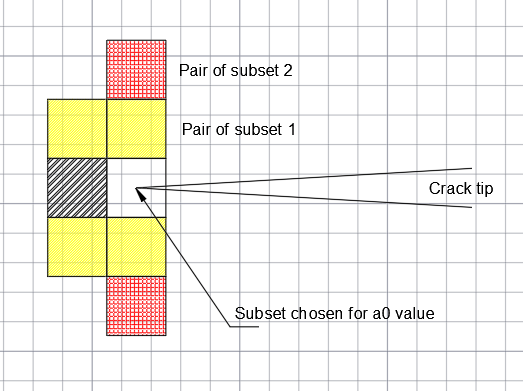
\includegraphics[width=8cm]{fig29bis}
	\caption{Pair of subsets around the chosen subset a0}
	\label{fig:fig29bis}
\end{figure}

\textbf{Mapping function and mapping mask}

The method used is based on the variation of the relative position between adjacent subsets which gives an estimate of the damage occurrence \cite{Xavieretal2014}. To begin with, a matching function A(x,y) \ref{eq:eq21} is determined based on the norm of the relative position vectors as follows:

\begin{equation}
	A(x,y)=max(\lVert u_i-u_k\rVert;\lVert u_j-u_l\rVert)
	\label{eq:eq21}
\end{equation}

where $u_{i,j,k,l}$ represent the displacement vector of four adjacent subsets. A mapping mask \ref{eq:eq22} is then defined assuming threshold segmentation according to the following inequalities.

\begin{equation}
	M(x,y)=
	\begin{cases}
		1 \text{ if } A(x,y) \geq \alpha \overline{A} \\
		0 \text{ if } A(x,y)< \alpha \overline{A}\\
		-1 \text{ if } A(x,y)= no data 
	\end{cases}
	\label{eq:eq22}
\end{equation}

The matrix M represents, for a given step, the length of the crack by having a larger value in the crack area. If the user looks too close, the noise of the values will prevent a good analysis, but looking too high on the matrix, the crack length value will not be accurate. To move around and get an accurate idea of how the user can look at the M matrix, it is important to use $\alpha$. The alpha parameter is like a cutting tool that allows one to get as close to the noise as possible without problems. Thus, when a subset is outside this region, it will be considered as zero. Then, subsets that are placed in the crack, or somewhere where there is a defect or missing information as in the crack, the subset will be defined with a value equal to -1. Then, for all the subsets around the crack, which have a real interest in the study, they will take the value equal to 1. Using this sub-step matrix, now composed of -1, 0, 1, it is possible to plot the whole matrix in shades of gray, and to have an overview of the crack development. So, by following the farthest 1 value in the matrix, it is possible to know the last subset where the crack tip is localized.

\textbf{$\alpha$ parameter}

It is important to determine the $\alpha$ parameter. This one is used on the matrix as the matrix M. It is a tricky part of the code.To approximate the $\alpha$ value, a first correlation factor is sought using the least squares regression method. Indeed, we know that during the test, there are 3 main zones on the Displacement-Force curve: a first linear one which corresponds to a stationary zone, a second one where the fracture propagates and finally a third one which corresponds to the specimen rupture. With this correlation factor we find the stage between the stationary zone and the Fracture Process Zone FPZ. Then, a second stage verification criterion from the displacement field processing is used to verify the correct stage of the FPZ.
Thanks to these two steps, we know the stage where there is the begining of the FPZ and the values which are possible for $\alpha$.
It is then possible to plot for different $\alpha$ all the stages of the crack propagation and have an idea on the $\alpha$ value needed to have the greatest a(t). Normally, the alpha chosen is the smallest. However, a curve with a simpler geometry is preferred if the length a(t) does not change.
A part of the code allows to check the length of the crack graphically by selecting a0 and af directly in Python. This allows some alphas that do not have the correct crack length to be eliminated directly.

\textbf{Crack length}

Another part of the code allows us to obtain a(t) as a function of alpha. This is done by focusing on the ZOI and the number of subsets that compose it. Through the matrix composed by each subset, the displacement field can be observed. It is obtained by calculating the distance between the center of a subset and its displacement from one image to another. To simplify the code, this calculation is not performed on each subset but only on the four corners. By calculating the distance between the opposite corners, the maximum displacement in x and the displacement in y are introduced in a last matrix. Finally, the value of a(t) is equal to $a_0$ set by the user in the database and to $\Delta a$ which is the value of the crack length, evolving in time under the effect of the applied force.

\subsection{Method 2: Crack propagation based on crack opening displacement provided by DIC}

Method 2 uses the crack opening along the entire length of the wooden specimen to determine the length of the crack (\cite{FilhoJ2022}). 

\textbf{Crack opening displacement (COD) or Virtual displacement}

From the reference and current positions of the DIC calculation points, the Euclidean distance between each pair of points can be measured and the COD can be determined as \ref{eq:eq23}:

\begin{equation}
	VD(k,i_n)=\sqrt{(x_{11bk}-x_{11tk})^2 + (x_{22bk}-x_{22tk})^2}_{i_n} - VD(k,i_0)
	\label{eq:eq23}
\end{equation}

where the indices t and b refer to the DIC data points located at the top and bottom of the crack path, k is the index of the DIC point, $i_n$ is the image captured at time n, VD(k, i0) is the initial Euclidean distance between the computational points of the top and bottom reference DIC subset obtained from image i0, and $x_{11}$ and $x_{22}$ are their coordinates in the image plane. VD can be defined as a displacement gauge along the crack path \ref{fig:fig30}.

\begin{figure}[htp]
	\centering
	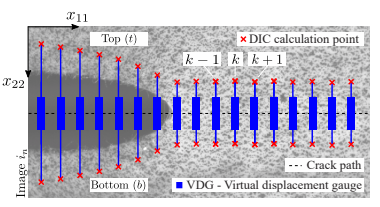
\includegraphics[width=10cm]{fig30}
	\caption{DIC-based virtual displacement gauge (VDG), \cite{FilhoJ2022}}
	\label{fig:fig30}
\end{figure}

\textbf{$\alpha$ and $\beta$ parameters}

The first step towards detecting the crack tip is to take the average value of VD for each stage, \ref{eq:eq24}:

\begin{equation}
	\overline{VD}(i_n)=\frac{1}{k} \sum_{k=1}^{k}VD(k,i_n)
	\label{eq:eq24}
\end{equation}

The threshold value must be adjusted using the two parameters $\alpha$ and $\beta$ which are obtained by solving the equation \ref{eq:eq25}:

\begin{equation}
	\begin{cases}
		VD_{th}(i_1)=\overline{VD}(i_1)(\alpha i_1 +\beta)\\
		VD_{th}(i_f)=\overline{VD}(i_f)(\alpha i_f +\beta)\\ 
	\end{cases}
\label{eq:eq25}
\end{equation}

In order to obtain $VD_{th}(i_1)$ and $VD_{th}(i_f)$, it was first necessary to read graphically the position of the crack tip of the first and last image and then to find the intersection between the position of the crack tip and the crack opening VD for those two stages.

Therefore, the adjusted threshold line-cut $VD_{th}(i_n)$ is given by \ref{eq:eq26}:

\begin{equation}
	VD_{th}(i_n)=\overline{VD}(i_n)(\alpha i_n +\beta)
	\label{eq:eq26}
\end{equation}

The intersection between each $VD_{th}(i_n)$ and the corresponding $VD(k, i_n)$ curve at time n represents the $x_{11}$ position of the crack tip, denoted by ($p_n$).
It is therefore possible to calculate the growth of the crack at instant n \ref{eq:eq27}:

\begin{equation}
	da_n=p_n-p_0
	\label{eq:eq27}
\end{equation}

\subsection{Difficulties in applying method 2}

This method was originally used for a fibrous soft material. The first step was to translate the Matlab code given by \cite{FilhoJ2022} into a python code to be able to use both methods simultaneously and compare them.
After translating the code, we realised that this method did not work properly for the wood material and the DIC data we had with Stanislas' tests.
From the data of method 1, we already know the position of a0 and all the displacements over time that have occurred on the entire wooden specimen. However, for method 2, we only need 2 horizontal lines placed above and below the fracture. It is therefore sufficient to take only one part of the data from the specimen. Moreover, it was chosen to take these two lines far enough away from the fracture in order not to have subsets without any data.
However, method 2 still didn't work properly and a slight modification to the code was required.

The figure \ref{fig:fig31} corresponds to the plot of $\overline{VD}$ and $VD_{th}$ with Joao's data, the author of the method. We read graphically $a_1$ and $a_f$, which allowed us to know the $VD_{th}$ for index 1 and the last index which are the bounds on the y-axis for the $VD_{th}$ curve. We notice that the $VD_{th}$ curve has the same shape as the $\overline{VD}$ curve, is still increasing but has only been reduced at the ordinate level. This is what we want to achieve for the MMCG specimens.

For the MMCG test data, by applying $VD_{th1}$ and $VD_{thf}$ as in Joao's data, we notice that the $VD_{th}$ curve increases and then decreases, which is not normal since the COD should normally increase with time (figure \ref{fig:fig32}). This is due to the alpha and beta factors which increase $\overline{VD}$ for the first indices and then decrease $\overline{VD}$ for the last indices. According to the equation \ref{eq:eq26} alpha is multiplied by $i_n$ which will decrease the multiplier coefficient of $\overline{VD}$ over time if alpha is negative and beta positive. This is the reason why $VD_{th}$ is under $\overline{VD}$  for the latest indices.

\begin{figure}[htp]
	\begin{minipage}[c]{.46\linewidth}
		\centering
		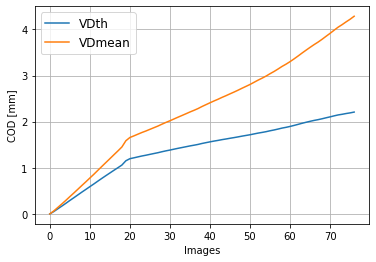
\includegraphics[width=7cm]{fig31}
		\caption{$\overline{VD}$ and $VD_{th}$ with Joao's data}
		\label{fig:fig31}
	\end{minipage}
	\hfill%
	\begin{minipage}[c]{.46\linewidth}
		\centering
		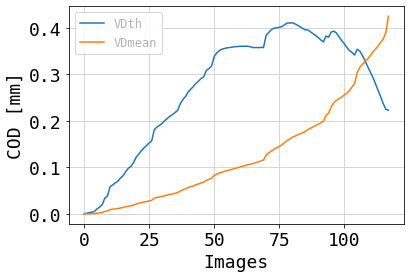
\includegraphics[width=7cm]{fig32}
		\caption{$\overline{VD}$ and $VD_{th}$ with stanislas' data}
		\label{fig:fig32}
	\end{minipage}
\end{figure}


Method 1 was then used to find out from which image the fracture process starts. Method 2 directly increased the length of the crack for the first images, which is not normally the case for wood.  Indeed, it is considered that for all the images before the FPZ there is a(t)=a0. We therefore read $a_1$ and $a_f$ with $a_1$ the index of the beginning of the fracture process and $a_f$ the last image before the material breaks. The graph \ref{fig:fig33} is then obtained.


\begin{figure}[htp]
	\centering
	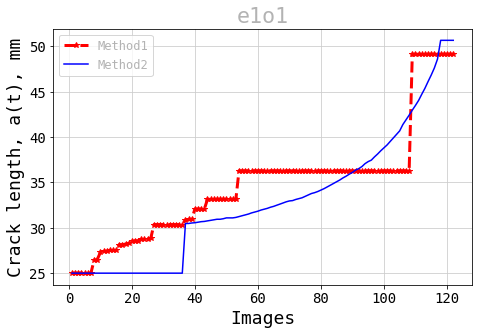
\includegraphics[width=7cm]{fig33}
	\caption{Crack length with FPZ taken into account}
	\label{fig:fig33}
\end{figure}

The fracture for method 2 starts much later than method 1 and are different over the time. Furthermore, the crack length does not end at the same place, because for method 2 the fracture at the last index is read graphically which is less accurate.
Because the $\overline{VD}$ is too small compared to the graphically obtained $VD_{th1}$, an interpolation is made to increase the $\overline{VD}$. The graph \ref{fig:fig34} is obtained:

\begin{figure}[htp]
	\centering
	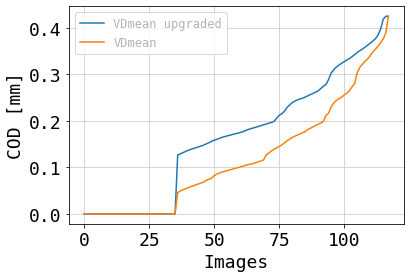
\includegraphics[width=7cm]{fig34}
	\caption{Interpolation of $\overline{VD}$}
	\label{fig:fig34}
\end{figure}

Thanks to this interpolation, we apply alpha and beta (figure \ref{fig:fig35}) and obtain $VD_{th}$. Finally, we obtain the crack length graph \ref{fig:fig36}:

\begin{figure}[h]
	\begin{minipage}[c]{.46\linewidth}
		\centering
		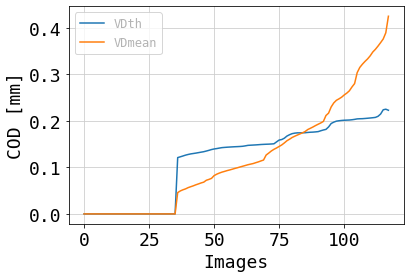
\includegraphics[width=7cm]{fig35}
		\caption{$VD_{th}$ with interpolation}
		\label{fig:fig35}
	\end{minipage}
	\hfill%
	\begin{minipage}[c]{.46\linewidth}
		\centering
		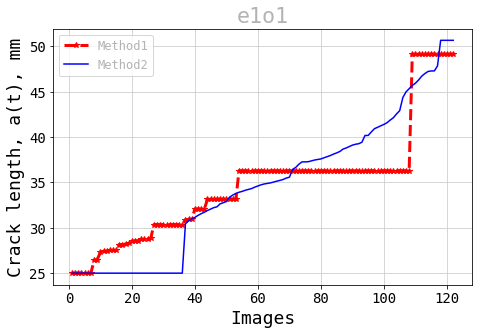
\includegraphics[width=7cm]{fig36}
		\caption{Final crack length e1o1}
		\label{fig:fig36}
	\end{minipage}
\end{figure}

To conclude, the crack propagation does not start at the same stage between the two methods and the crack length is different over the time. Moreover we had to modify a lot Joao's initial method to apply it to wood material. It also adds uncertainties since we have to read graphically $a_1$ and $a_f$ to obtain the crack length thresholds at the beginning and at the end of the propagation. Reading the points $a_1$ and $a_f$ is really difficult to evaluate manually for this material because the fracture is not clearly visible on the images. In addition, the index for $a_1$ and $a_f$ is given by method 1 which adds further uncertainties. Method 2 gives a "smoother" curve than method 1, but this is not necessarily a good thing since the fracture of wood material usually works in fits and starts.
As observed in method 1, the fracture process typically involves multiple stages, which can be attributed to the gradual propagation of cracks. In some instances, the presence of bridges in the material can impede the linear advancement of the crack. However, once these bridges break, the crack can propagate further, resulting in the development of a new stage in the fracture process. This underscores the complex nature of crack propagation in wood. In the next chapter, the tests carried out in mode I will be presented and we will be able to check whether method 2 works correctly with wood. However, some doubts are raised, as the $\overline{VD}$ is not as linear as with a soft fibrous material, as shown in figures \ref{fig:fig31} and \ref{fig:fig32}.

\subsection{Energy restitution rate}

After using one of the two previous methods, we can calculate the energy restitution rate in mode I and in mixed mode.

For mode I, the formula is the one explained in \ref{eq:eq125}.

For mixed mode, the formula becomes \ref{eq:eq28}:

\begin{equation}
	\begin{cases}
		G_I=\frac{{F_{cy}}^2}{2b}\ \frac{\partial C_I}{\partial a} \quad \text{with } C_I=\frac{v}{F_{cy}} \\
		G_{II}=\frac{{F_{cx}}^2}{2b}\ \frac{\partial C_{II}}{\partial a} \quad \text{with } C_{II}=\frac{u}{F_{cx}}\\ 
	\end{cases}
\label{eq:eq28}
\end{equation}

where u and v are the crack opening displacement according to x and y. The displacement measured by the machine is not used to calculate the energy restitution rate, as it is less accurate due to the clearances in the jaws.

In mixed mode the camera will have the same inclination as the specimen figure \ref{fig:fig37bis}.

\begin{figure}[htp]
	\centering
	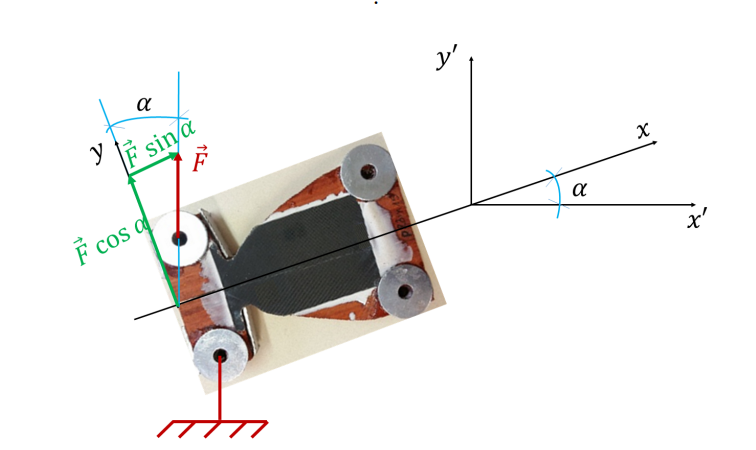
\includegraphics[width=9cm]{fig37bis}
	\caption{Force projection along the axes in mixed mode, \cite{Odounga2018phd}}
	\label{fig:fig37bis}
\end{figure}

The crack opening values will therefore be projected directly along the x and y axes. The force is projected along the x and y axes, so we have \ref{eq:eq29}:


\begin{equation}
	\begin{cases}
		F_{cx}=F \sin(\alpha) \\
		F_{cy}=F \cos(\alpha) \\ 
	\end{cases}
	\label{eq:eq29}
\end{equation}


\section{Specimen preparation}

\subsection{Specimen names}

We have 20 specimens of silver fir of 12.5mm thickness.
We will therefore use 5 specimens per degree of inclination. This means 5 specimens in pure mode I (0°) and 15 specimens in mixed mode (15°, 30°, and 45°).
Naming the specimens allows to know which test was performed on which specimen. The first part of the name corresponds to the inclination of the specimen during the test using the Arcan system:
\newline
E0 : Test in pure mode I
\newline
E15 : Test with specimen tilt of 15°
\newline
E30 : Test with specimen tilt of 30°
\newline
E45 : Test with specimen tilt of 45°


E15, E30 and E45 are therefore the specimens tested in mixed mode.
Then the name as a second component is the number of the specimen dedicated to this test.
Finally, all samples are named as E0E1 which is the first sample used in pure mode.

\subsection{Notch and precrack}

Notches were created in each specimen. A precrack is made by a cutter into the notch. The interest is to initiate a straight crack, thanks to this first one. The notch width is around 1.5mm, done by a straight electrical saw. The cutter allow to go deeper and create a precrack with a shape that allows the propagation of the crack. The precrack must be done at the center of the sample heel. Indeed, even a little eccentricity could cause a deviation of the crack and prevent a good study of the propagation. The specimen was designed with an initial crack noted $a_i$ and the total crack length is equal to: $a=a_i+\Delta a$.

The initial crack lengths are obtained by averaging the notch on each side of the specimen plus the precrack also measured with the average of the two sides of the specimen.
The following initial crack length values are then obtained:

\begin{table}[h]
	\centering
	\begin{tabular}{c c }
		\multicolumn{1}{l}{} & \multicolumn{1}{l}{Initial Crack length} \\
		\multicolumn{1}{c}{\cellcolor[HTML]{F8CBAD}E0E1} & 25,3   mm \\
		\multicolumn{1}{c}{\cellcolor[HTML]{F8CBAD}E0E2} & 24.85 mm \\
		\multicolumn{1}{c}{\cellcolor[HTML]{F8CBAD}E0E3} & 25.65 mm \\
		\multicolumn{1}{c}{\cellcolor[HTML]{F8CBAD}E0E4} & 24,7 mm \\ 
		\cellcolor[HTML]{F8CBAD}E0E5 & 25,6 mm \\ 
		\cellcolor[HTML]{F8CBAD}E0E6 & 26,3 mm \\ 
		\multicolumn{1}{c}{\cellcolor[HTML]{C65911}E15E1} & 25,85 mm \\ 
		\multicolumn{1}{c}{\cellcolor[HTML]{C65911}E15E2} & 25,6 mm \\ 
		\multicolumn{1}{c}{\cellcolor[HTML]{C65911}E15E3} & 25,55 mm \\ 
		\multicolumn{1}{c}{\cellcolor[HTML]{C65911}E15E4} & 25.3 mm \\
		\multicolumn{1}{c}{\cellcolor[HTML]{C65911}E15E5} & 24,85 mm \\ 
		\multicolumn{1}{c}{\cellcolor[HTML]{BF8F00}E30E1} & 25,55 mm \\ 
		\multicolumn{1}{c}{\cellcolor[HTML]{BF8F00}E30E2} & 24,4 mm \\ 
		\multicolumn{1}{c}{\cellcolor[HTML]{BF8F00}E30E3} & 24,2 mm \\ 
		\multicolumn{1}{c}{\cellcolor[HTML]{BF8F00}E30E4} & 25,3 mm \\ 
		\multicolumn{1}{c}{\cellcolor[HTML]{BF8F00}E30E5} & 24.4 mm \\ 
		\multicolumn{1}{c}{\cellcolor[HTML]{BF8F00}E30E6} & 24.35 mm \\ 
		\multicolumn{1}{c}{\cellcolor[HTML]{BF8F00}E30E7} & 25.6 mm \\
		\multicolumn{1}{c}{\cellcolor[HTML]{FFA500}E45E1} & 25,8 mm \\ 
		\multicolumn{1}{c}{\cellcolor[HTML]{00FF00}broken} & 25.95 mm \\  
	\end{tabular}
	\caption{Precrack dimensions}
	\label{tab:Tab11}
\end{table}

We can see that only one test was carried out at 45 degrees. Some tests were not successful. The tests for angles 0°, 15° and 30° were therefore preferred.

\section{Conclusion}

This chapter has given us a better understanding of all the tools used to carry out the tests. It also explains some parameters that are essential to the success of the DIC method. Finally, it presents two methods for evaluating crack length; one using full-field displacement and the other using COD.
According to the results from the two methods, method 1 appears to be more accurate than method 2. In the next chapter, we will be able to better evaluate the efficiency of the two methods.


